\documentclass[UTF8,a4paper,12pt]{ctexart}

\usepackage[left=2.2cm,right=2.2cm,top=2.5cm,bottom=2.5cm]{geometry}
\usepackage{graphicx}
\usepackage{booktabs}
\usepackage{amsmath}
\usepackage{amssymb}
\usepackage{float}
\usepackage{hyperref}
\usepackage{caption}
\usepackage{array}

\hypersetup{
    colorlinks=true,
    linkcolor=black,
    urlcolor=blue,
    citecolor=black
}

\graphicspath{{figures/}}
\title{HW1 实验报告\\从零开始构建三层神经网络分类器实现 Fashion-MNIST 图像分类}
\author{课程：计算机视觉}
\date{\today}

\begin{document}

\maketitle

\section{实验目标}

本次作业要求在不依赖 PyTorch、TensorFlow、JAX 等自动微分框架的前提下，仅使用 \texttt{NumPy} 手工实现一个三层神经网络分类器，在 Fashion-MNIST 数据集上完成训练、验证、测试与结果分析。按照作业 PDF 的要求，最终实现需要覆盖以下内容：

\begin{itemize}
    \item 数据加载与预处理；
    \item 模型定义与反向传播；
    \item SGD、学习率衰减、交叉熵损失与 L2 正则；
    \item 超参数搜索与最优模型保存；
    \item 独立测试集准确率与混淆矩阵；
    \item 训练曲线、第一层权重可视化与错例分析；
    \item README、代码仓库链接与模型权重下载链接。
\end{itemize}

\section{方法设计}

\subsection{数据集与预处理}

Fashion-MNIST 包含 10 个服装类别，每张图像为 $28 \times 28$ 的灰度图。代码中将每张图像拉平成 784 维向量后输入 MLP。数据集划分方式如下：

\begin{itemize}
    \item 训练集：54000 张；
    \item 验证集：6000 张；
    \item 测试集：10000 张。
\end{itemize}

预处理步骤较简单：

\begin{itemize}
    \item 将像素值归一化到 $[0,1]$；
    \item 训练阶段按 batch 随机打乱；
    \item 验证集与测试集按固定顺序评估。
\end{itemize}

\subsection{模型结构}

本实验实现的是一个两层隐藏层、三层线性层的 MLP：

\begin{equation}
    x \in \mathbb{R}^{784}
    \rightarrow \text{Linear}(784, h)
    \rightarrow \text{Activation}
    \rightarrow \text{Linear}(h, h)
    \rightarrow \text{Activation}
    \rightarrow \text{Linear}(h, 10)
\end{equation}

其中隐藏维度 $h$ 可调，激活函数支持 \texttt{ReLU}、\texttt{Sigmoid} 和 \texttt{Tanh}。本次最优模型采用 \texttt{ReLU} 和 $h=1024$。

以最终配置为例，模型参数量为：

\begin{equation}
784 \times 1024 + 1024 + 1024 \times 1024 + 1024 + 1024 \times 10 + 10 = 1{,}863{,}690
\end{equation}

\subsection{反向传播与优化}

整个训练过程没有使用自动微分框架，而是为每一层显式实现前向与反向传播：

\begin{itemize}
    \item 线性层保存输入并在反向传播时计算 $\partial L / \partial W$、$\partial L / \partial b$ 与 $\partial L / \partial x$；
    \item ReLU、Sigmoid、Tanh 分别实现对应的梯度传播；
    \item 损失函数采用 Softmax + Cross-Entropy；
    \item 优化器采用 SGD，并在权重项上加入 L2 正则；
    \item 每个 epoch 结束后使用学习率衰减：$lr \leftarrow lr \times lr\_decay$。
\end{itemize}

训练时以验证集准确率作为模型选择标准，只要验证集准确率提升，就将当前权重保存为 \texttt{checkpoints/best\_model.pkl}。

\section{代码结构}

仓库中的核心模块与作业要求一一对应：

\begin{itemize}
    \item \texttt{src/dataloader.py}：数据读取、归一化、训练/验证划分、batch 生成；
    \item \texttt{src/layers.py}：线性层与激活函数；
    \item \texttt{src/model.py}：三层 MLP 封装；
    \item \texttt{src/loss.py}：Softmax Cross-Entropy；
    \item \texttt{src/optimizer.py}：SGD、Weight Decay、Learning Rate Decay；
    \item \texttt{train.py}：训练与最优模型保存；
    \item \texttt{search\_param.py}：网格搜索；
    \item \texttt{test.py}：测试集准确率、混淆矩阵与结果保存；
    \item \texttt{main.py}：完整 pipeline。
\end{itemize}

\section{实验设置}

\subsection{超参数搜索}

搜索空间如下：

\begin{itemize}
    \item 学习率：$\{10^{-2}, 10^{-3}, 10^{-4}\}$；
    \item 隐藏层维度：$\{128, 256, 512, 1024\}$；
    \item L2 正则强度：$\{10^{-3}, 10^{-4}, 10^{-5}\}$；
    \item 每组搜索配置训练 30 个 epoch；
    \item batch size 固定为 512，激活函数固定为 ReLU。
\end{itemize}

完整搜索结果见 \texttt{report/grid\_search\_results.txt}。表 \ref{tab:grid} 展示其中几组代表性结果。

\begin{table}[H]
    \centering
    \caption{代表性超参数搜索结果}
    \label{tab:grid}
    \begin{tabular}{cccc}
        \toprule
        学习率 & 隐藏层维度 & Weight Decay & 验证集准确率 \\
        \midrule
        0.01   & 128  & $10^{-4}$ & 0.8457 \\
        0.01   & 512  & $10^{-5}$ & 0.8475 \\
        0.01   & 1024 & $10^{-5}$ & 0.8507 \\
        0.01   & 1024 & $10^{-4}$ & \textbf{0.8518} \\
        0.001  & 1024 & $10^{-5}$ & 0.7708 \\
        0.0001 & 1024 & $10^{-3}$ & 0.6193 \\
        \bottomrule
    \end{tabular}
\end{table}

从搜索结果可以得到三点结论：

\begin{itemize}
    \item 学习率 $0.01$ 明显优于 $0.001$ 和 $0.0001$，后两者存在明显欠拟合；
    \item 隐藏层维度增大通常能稳定提升性能，1024 的结果最好；
    \item 正则强度过大（如 $10^{-3}$）会压制模型表达能力，而 $10^{-4}$ 或 $10^{-5}$ 更合适。
\end{itemize}

\subsection{最终训练配置}

根据网格搜索结果，最终模型使用如下配置重新训练 500 个 epoch：

\begin{table}[H]
    \centering
    \caption{最终训练配置}
    \begin{tabular}{cc}
        \toprule
        项目 & 数值 \\
        \midrule
        Hidden Dimension & 1024 \\
        Activation & ReLU \\
        Learning Rate & 0.01 \\
        Weight Decay & 0.0001 \\
        LR Decay & 0.95 \\
        Batch Size & 512 \\
        Epochs & 500 \\
        \bottomrule
    \end{tabular}
\end{table}

\section{实验结果}

\subsection{训练曲线}

图 \ref{fig:curves} 给出了训练集与验证集上的 Loss 曲线，以及验证集 Accuracy 曲线。可以看到：

\begin{itemize}
    \item 训练初期收敛较快，前几十个 epoch 内损失迅速下降；
    \item 验证集准确率在约 0.85 附近稳定；
    \item 后期曲线基本趋于平稳，说明模型已经充分收敛。
\end{itemize}

\begin{figure}[H]
    \centering
    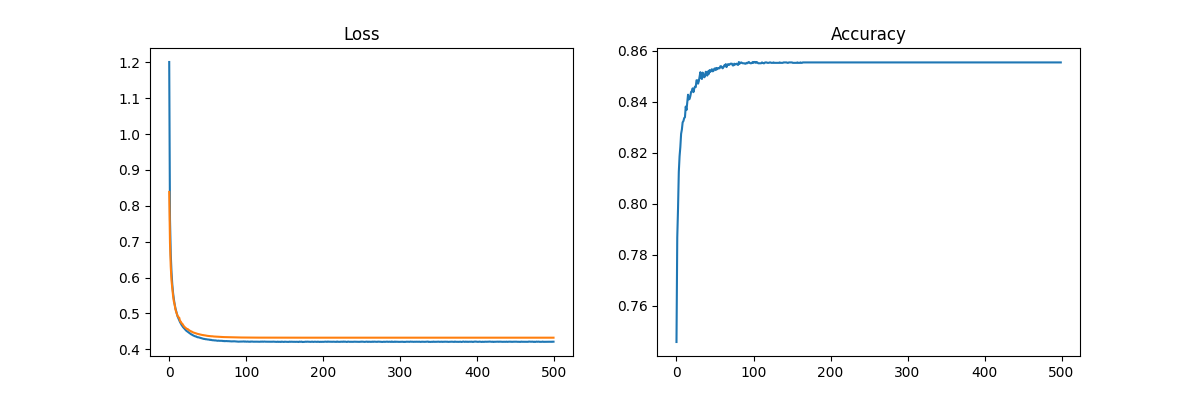
\includegraphics[width=0.92\textwidth]{curves.png}
    \caption{训练集/验证集 Loss 曲线与验证集 Accuracy 曲线}
    \label{fig:curves}
\end{figure}

\subsection{测试集准确率与混淆矩阵}

当前仓库中最佳权重文件 \texttt{checkpoints/best\_model.pkl} 在测试集上的结果为：

\begin{itemize}
    \item 测试集准确率：\textbf{0.8422}；
    \item 结果文本已保存至 \texttt{results/test\_metrics.txt}；
    \item 混淆矩阵图已保存至 \texttt{results/confusion\_matrix.png}。
\end{itemize}

\begin{figure}[H]
    \centering
    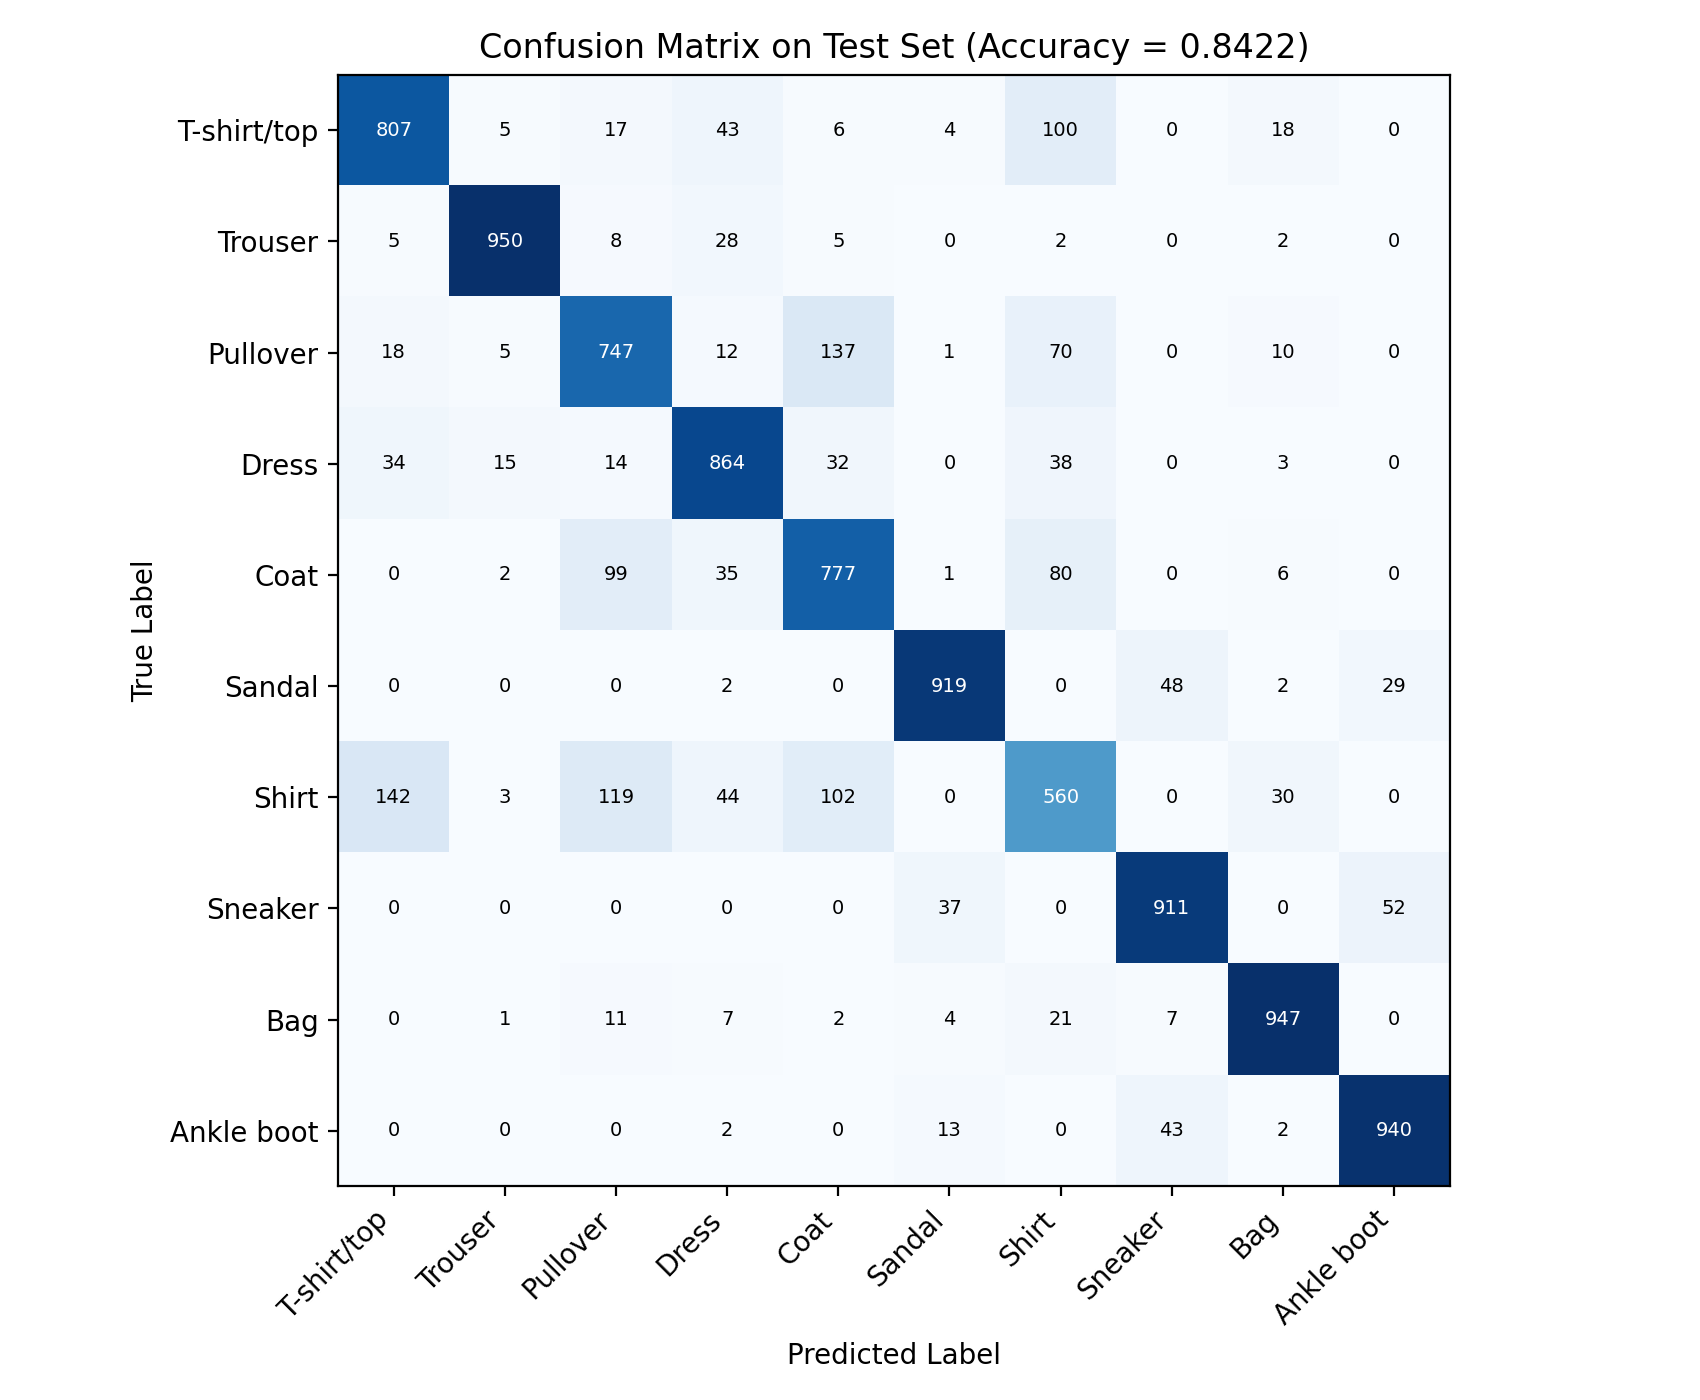
\includegraphics[width=0.88\textwidth]{confusion_matrix.png}
    \caption{测试集混淆矩阵}
    \label{fig:cm}
\end{figure}

从混淆矩阵中可以看出，模型最容易混淆的类别主要集中在外观相近的上衣类与鞋类：

\begin{itemize}
    \item \texttt{Shirt} 容易被分成 \texttt{T-shirt/top}、\texttt{Pullover}、\texttt{Coat}；
    \item \texttt{Pullover} 与 \texttt{Coat} 之间混淆较明显；
    \item \texttt{Sneaker}、\texttt{Sandal}、\texttt{Ankle boot} 三类鞋类之间也存在一定误判。
\end{itemize}

这与 Fashion-MNIST 的低分辨率特点一致：许多类别只在袖型、衣摆、鞋帮高度等细节上存在差异，而 MLP 直接处理展平后的像素向量，缺少卷积网络那样的局部结构先验，因此更容易在局部形态接近的类别之间混淆。

\subsection{第一层权重可视化与空间模式观察}

按照作业要求，将第一层线性层的权重恢复为 $28 \times 28$ 图像进行可视化，如图 \ref{fig:weights} 所示。

\begin{figure}[H]
    \centering
    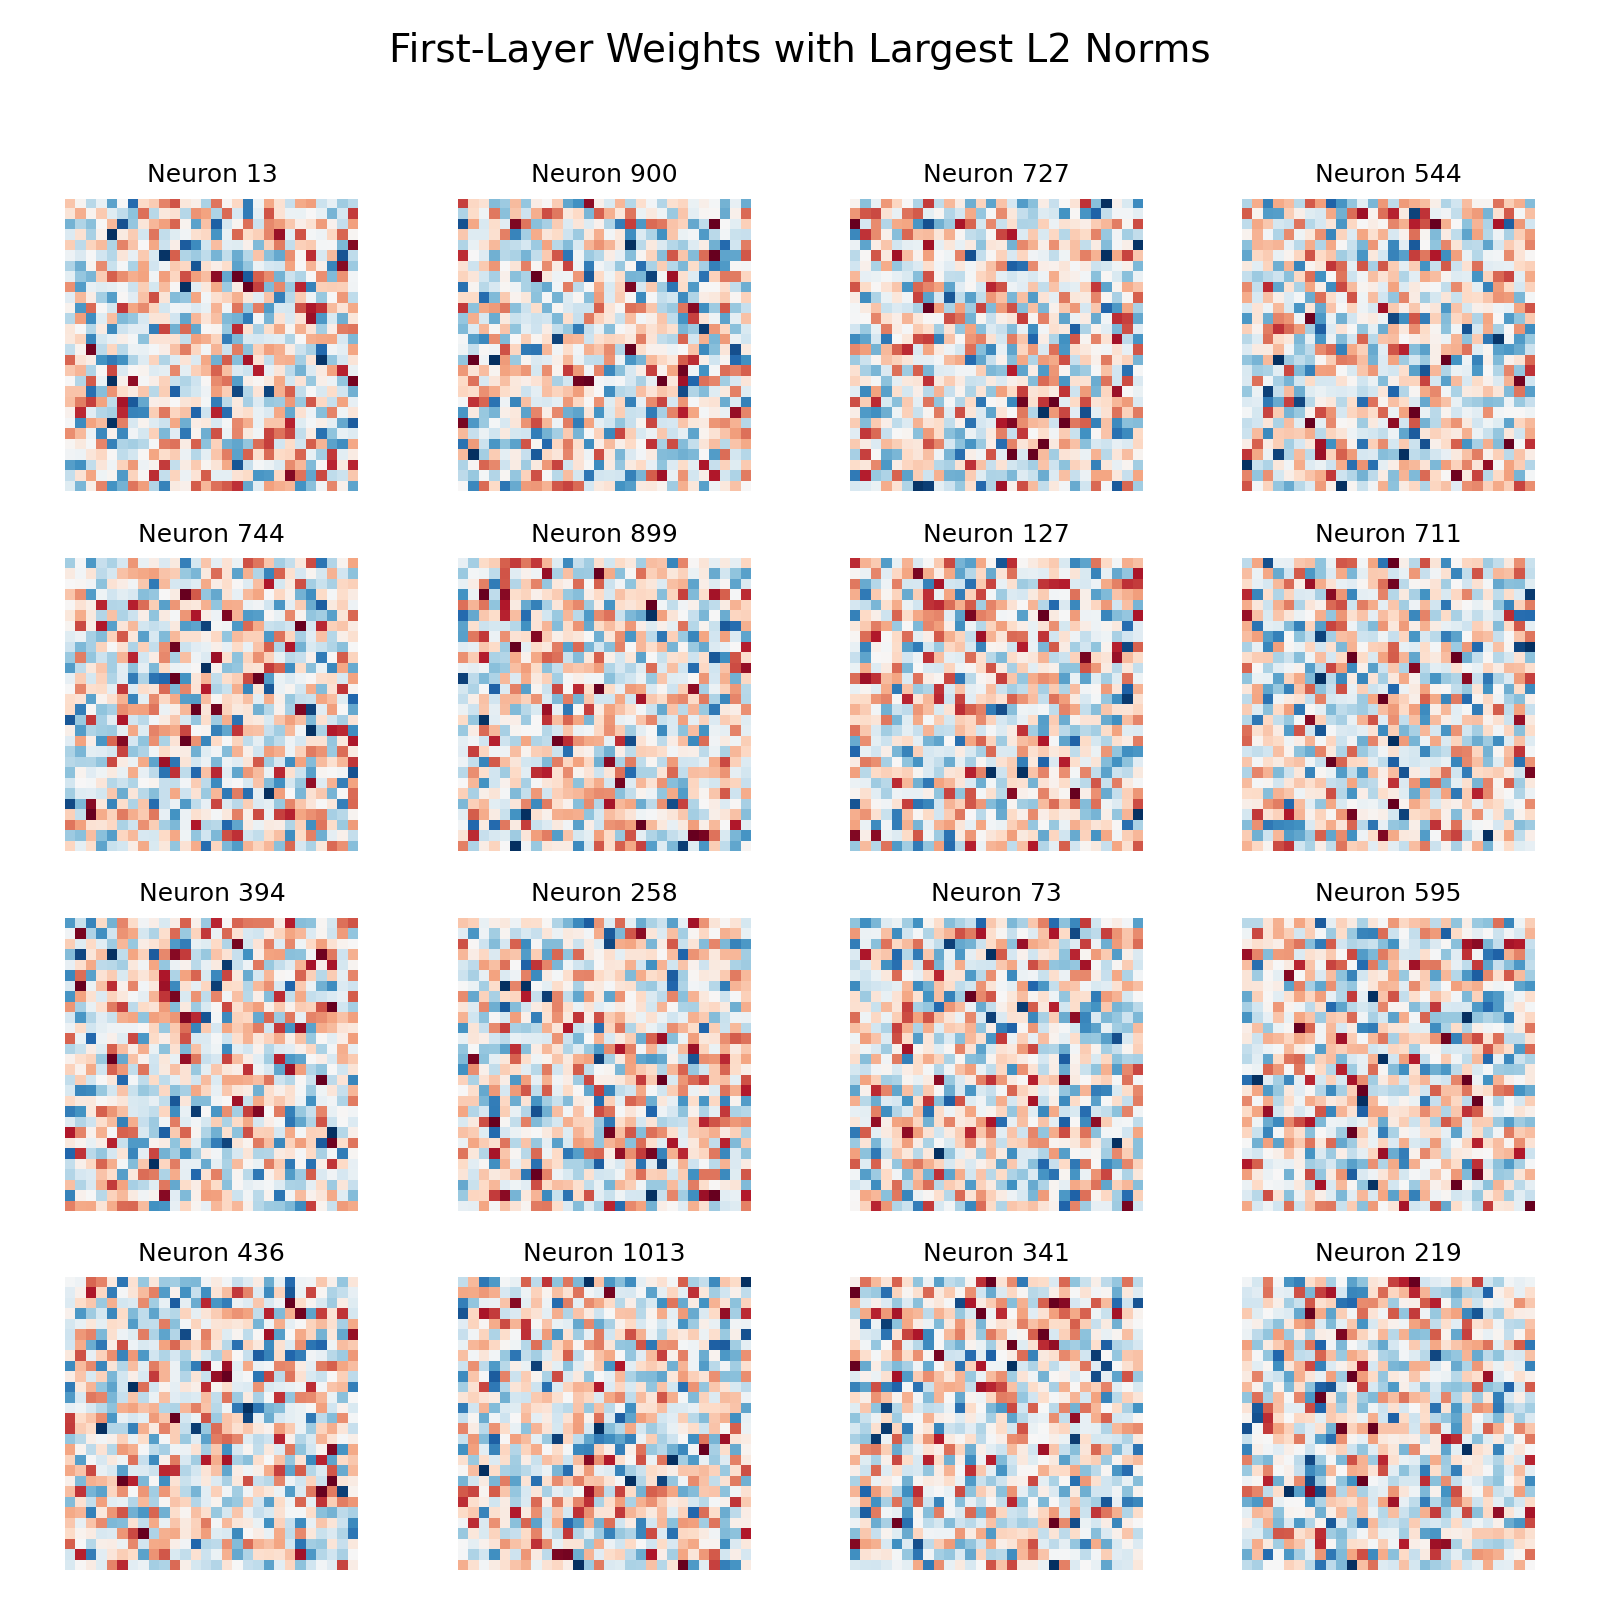
\includegraphics[width=0.86\textwidth]{weights_improved.png}
    \caption{第一层隐藏层权重可视化}
    \label{fig:weights}
\end{figure}

从可视化结果可以观察到以下现象：

\begin{itemize}
    \item 部分神经元已经出现了较弱的正负响应区域，说明模型开始利用图像的整体空间分布来区分类别；
    \item 某些权重在图像中心、上半部分或下半部分更活跃，这对应服装上身轮廓、下摆位置或鞋底区域等粗粒度结构；
    \item 与 CNN 常见的清晰边缘检测器不同，这里的权重图整体更分散、更噪声化，说明展平后的 MLP 虽然能学习到空间偏好，但难以形成稳定、局部化的边缘模板。
\end{itemize}

因此，本模型确实学到了一些与服装轮廓和空间分布有关的模式，但这些模式更偏向全局统计而不是明确的局部边缘特征。这也是 MLP 在图像任务上通常不如卷积结构高效的重要原因。

\subsection{错例分析}

图 \ref{fig:error} 展示了测试集中 5 个分类错误样本。

\begin{figure}[H]
    \centering
    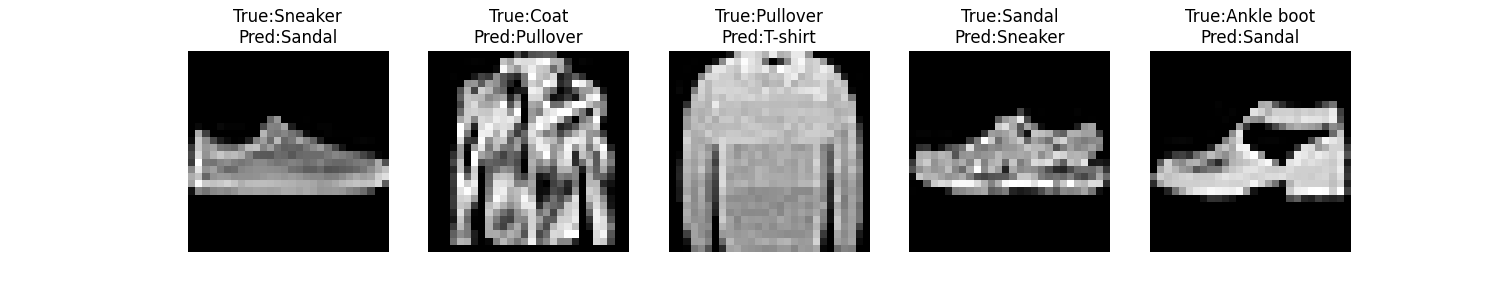
\includegraphics[width=\textwidth]{errors.png}
    \caption{测试集错例分析}
    \label{fig:error}
\end{figure}

结合图像内容与混淆矩阵，可对错例原因作如下分析：

\begin{itemize}
    \item \texttt{Sneaker} 被错分为 \texttt{Sandal}：由于图像中鞋面较低、轮廓较扁平，在 $28 \times 28$ 分辨率下高帮与开口结构不够明显；
    \item \texttt{Coat} 被错分为 \texttt{Pullover}：两者都呈现长袖上衣轮廓，而纽扣、领口、开襟等关键细节在低分辨率下很容易丢失；
    \item \texttt{Pullover} 被错分为 \texttt{T-shirt/top}：样本的袖口和衣身边界不够清楚，模型更多依赖整体灰度分布而非服装细节；
    \item \texttt{Ankle boot} 被错分为 \texttt{Sandal} 或 \texttt{Sneaker}：如果鞋帮部分与背景对比度较低，模型会更依赖鞋底与主体轮廓进行判断，从而造成误分。
\end{itemize}

总体来看，错例主要来自两类问题：一类是类别本身视觉相似，另一类是 Fashion-MNIST 分辨率较低，使得对分类至关重要的局部结构难以稳定保留。

\section{复现方式与提交信息}

本仓库支持以下复现命令：

\begin{itemize}
    \item \texttt{python search\_param.py}：执行超参数搜索；
    \item \texttt{python train.py}：使用默认最佳配置重新训练；
    \item \texttt{python test.py}：评估测试集并保存准确率与混淆矩阵；
    \item \texttt{python main.py}：执行完整 pipeline。
\end{itemize}

根据作业要求，实验报告中给出代码仓库与模型权重链接如下：

\begin{itemize}
    \item GitHub Repo：\href{https://github.com/Loong-C/FDU-Computer-Vision.git}{https://github.com/Loong-C/FDU-Computer-Vision.git}
    \item 模型权重下载：\href{https://drive.google.com/file/d/12k378k0q2_tA5KuZpSIs9tKtFYN-TZNC/view?usp=drive_link}{Google Drive 权重链接}
\end{itemize}

\section{总结}

本实验基于 \texttt{NumPy} 从零实现了一个三层 MLP 分类器，完整覆盖了数据处理、前向计算、反向传播、优化器、超参数搜索、最优模型保存、测试集评估、权重可视化和错例分析等要求。最终模型在 Fashion-MNIST 测试集上达到 \textbf{84.22\%} 的准确率。

实验结果表明，纯 MLP 在该任务上已经能够学习到一定的服装空间分布模式，但由于缺少局部连接与平移不变性先验，其权重模式较分散，对外观相近类别的区分能力有限。后续若采用卷积结构，通常可以得到更清晰的局部特征和更高的分类性能。

\end{document}
